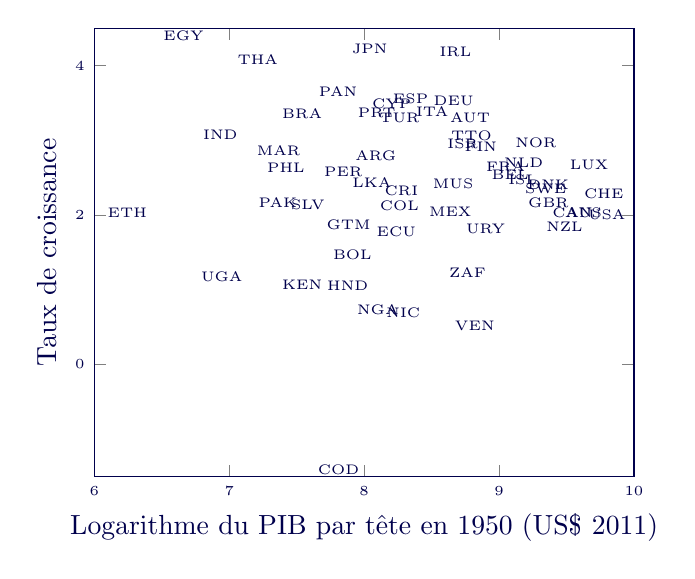
\begin{tikzpicture}
\tikzstyle{every node}=[font=\tiny]
\begin{axis}[
enlargelimits=false, color=blue!30!black,
scale=1,
xmin=6,
xmax=10,
xlabel style={font=\color{white!15!black}},
xlabel={Logarithme du PIB par tête en 1950 (US\$ 2011)},
ymin=-1.5,
ymax=4.5,
ylabel style={font=\color{white!15!black}},
ylabel={Taux de croissance},
axis background/.style={fill=white}
]
\node[right, align=left]
at (axis cs:7.863,2.793) {ARG};
\node[right, align=left]
at (axis cs:9.416,2.036) {AUS};
\node[right, align=left]
at (axis cs:8.565,3.297) {AUT};
\node[right, align=left]
at (axis cs:8.873,2.54) {BEL};
\node[right, align=left]
at (axis cs:7.697,1.466) {BOL};
\node[right, align=left]
at (axis cs:7.32,3.359) {BRA};
\node[right, align=left]
at (axis cs:9.322,2.027) {CAN};
\node[right, align=left]
at (axis cs:9.559,2.281) {CHE};
\node[right, align=left]
at (axis cs:7.585,-1.41) {COD};
\node[right, align=left]
at (axis cs:8.045,2.13) {COL};
\node[right, align=left]
at (axis cs:8.08,2.323) {CRI};
\node[right, align=left]
at (axis cs:7.987,3.486) {CYP};
\node[right, align=left]
at (axis cs:8.443,3.533) {DEU};
\node[right, align=left]
at (axis cs:9.138,2.41) {DNK};
\node[right, align=left]
at (axis cs:8.021,1.773) {ECU};
\node[right, align=left]
at (axis cs:6.44,4.398) {EGY};
\node[right, align=left]
at (axis cs:8.141,3.557) {ESP};
\node[right, align=left]
at (axis cs:6.026,2.029) {ETH};
\node[right, align=left]
at (axis cs:8.672,2.909) {FIN};
\node[right, align=left]
at (axis cs:8.832,2.648) {FRA};
\node[right, align=left]
at (axis cs:9.144,2.159) {GBR};
\node[right, align=left]
at (axis cs:7.65,1.868) {GTM};
\node[right, align=left]
at (axis cs:7.654,1.053) {HND};
\node[right, align=left]
at (axis cs:6.735,3.08) {IND};
\node[right, align=left]
at (axis cs:8.487,4.19) {IRL};
\node[right, align=left]
at (axis cs:8.997,2.466) {ISL};
\node[right, align=left]
at (axis cs:8.545,2.956) {ISR};
\node[right, align=left]
at (axis cs:8.313,3.388) {ITA};
\node[right, align=left]
at (axis cs:7.836,4.221) {JPN};
\node[right, align=left]
at (axis cs:7.319,1.067) {KEN};
\node[right, align=left]
at (axis cs:7.841,2.429) {LKA};
\node[right, align=left]
at (axis cs:9.452,2.673) {LUX};
\node[right, align=left]
at (axis cs:7.133,2.856) {MAR};
\node[right, align=left]
at (axis cs:8.409,2.042) {MEX};
\node[right, align=left]
at (axis cs:8.438,2.413) {MUS};
\node[right, align=left]
at (axis cs:7.876,0.729) {NGA};
\node[right, align=left]
at (axis cs:8.093,0.697) {NIC};
\node[right, align=left]
at (axis cs:8.966,2.697) {NLD};
\node[right, align=left]
at (axis cs:9.049,2.973) {NOR};
\node[right, align=left]
at (axis cs:9.278,1.849) {NZL};
\node[right, align=left]
at (axis cs:7.145,2.159) {PAK};
\node[right, align=left]
at (axis cs:7.593,3.651) {PAN};
\node[right, align=left]
at (axis cs:7.631,2.581) {PER};
\node[right, align=left]
at (axis cs:7.209,2.626) {PHL};
\node[right, align=left]
at (axis cs:7.882,3.364) {PRT};
\node[right, align=left]
at (axis cs:7.386,2.138) {SLV};
\node[right, align=left]
at (axis cs:9.12,2.352) {SWE};
\node[right, align=left]
at (axis cs:6.989,4.073) {THA};
\node[right, align=left]
at (axis cs:8.572,3.06) {TTO};
\node[right, align=left]
at (axis cs:8.04,3.297) {TUR};
\node[right, align=left]
at (axis cs:6.719,1.168) {UGA};
\node[right, align=left]
at (axis cs:8.683,1.818) {URY};
\node[right, align=left]
at (axis cs:9.587,1.997) {USA};
\node[right, align=left]
at (axis cs:8.601,0.52) {VEN};
\node[right, align=left]
at (axis cs:8.557,1.223) {ZAF};
\end{axis}
\end{tikzpicture}
%%% Local Variables:
%%% mode: latex
%%% TeX-master: t
%%% End:
